\documentclass[tikz,border=8pt]{standalone}
\usepackage{amsmath,amssymb}
\usetikzlibrary{arrows.meta,calc,decorations.markings,decorations.pathmorphing,patterns,shapes.geometric,positioning}

\begin{document}
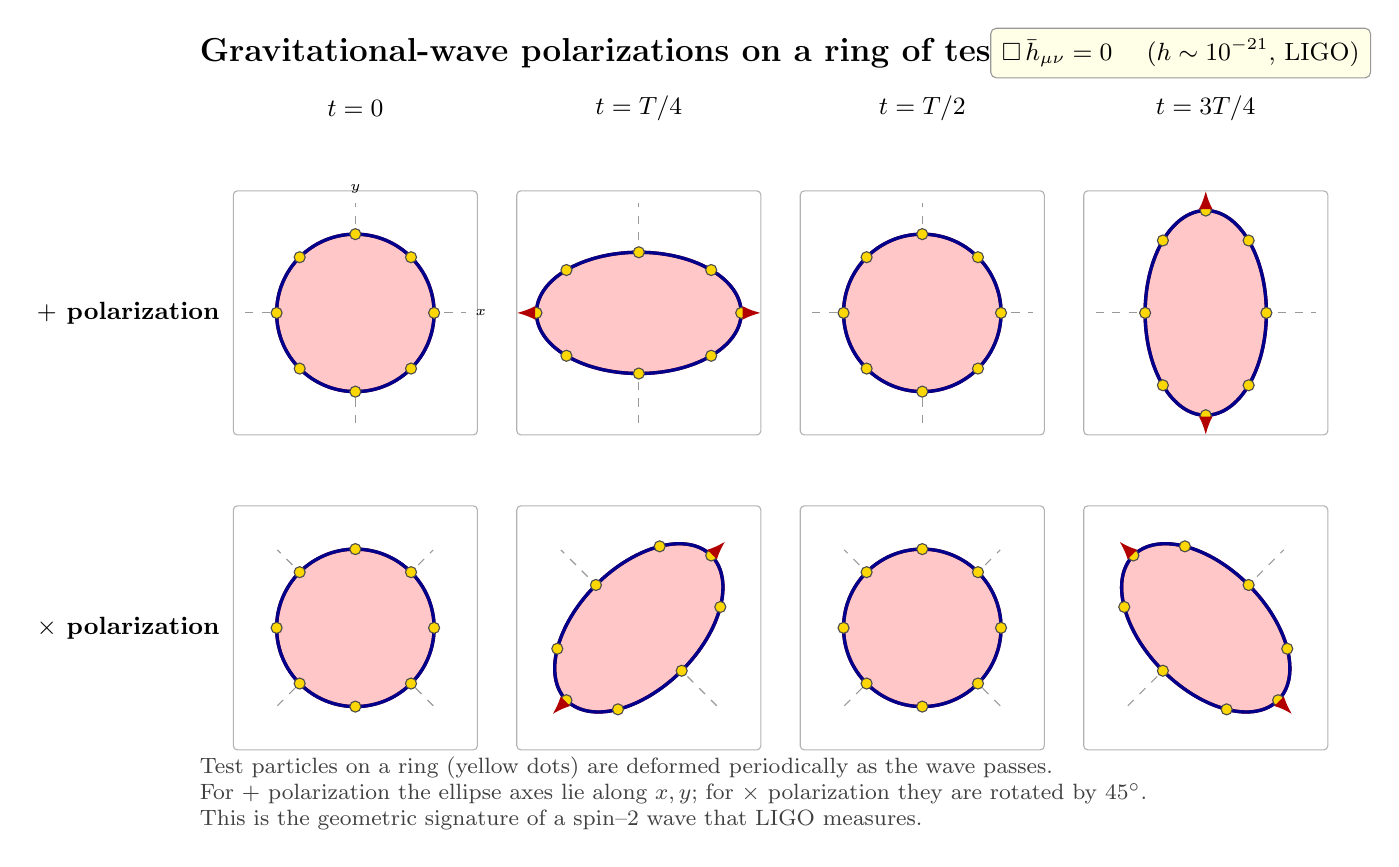
\begin{tikzpicture}[>=Latex,
  ringline/.style={draw=blue!55!black, very thick},
  ringfill/.style={fill=red!22!white, draw=red!55!black, very thick},
  particle/.style={circle, fill=yellow!75!orange, draw=black!70, thin, inner sep=0pt, minimum size=4pt},
  axisline/.style={draw=black!40, thin, dashed},
  framebox/.style={draw=black!30, thin, rounded corners=1.5pt}]

  % --- Title -----------------------------------------------------------------
  \node[font=\large\bfseries, anchor=west] at (-7.5, 5.7)
    {Gravitational-wave polarizations on a ring of test particles};

  % Equation labels (top-right)
  \node[font=\small, draw=black!40, rounded corners=2pt, fill=yellow!10, inner sep=4pt, anchor=east]
    at (7.5, 5.7) {$\Box\,\bar h_{\mu\nu} = 0$ \quad ($h\sim 10^{-21}$, LIGO)};

  % Column header time labels (placed once at the very top)
  \foreach \k/\lbl [count=\i from 0] in {0/{$t=0$}, 1/{$t=T/4$}, 2/{$t=T/2$}, 3/{$t=3T/4$}} {
    \node[font=\small\bfseries] at ($(-5.4 + 3.6*\k, 5.0)$) {\lbl};
  }

  % Row labels (left side)
  \node[font=\small\bfseries, anchor=east, align=right]
    at (-7.0, 2.4) {$+$ polarization};
  \node[font=\small\bfseries, anchor=east, align=right]
    at (-7.0, -1.6) {$\times$ polarization};

  % ---------------------------------------------------------------------------
  % Helper: a single panel.
  % parameters supplied via pgfmath: \cx (center x), \cy (center y),
  %   \rx (semi-axis x), \ry (semi-axis y), \rot (rotation in degrees)
  % ---------------------------------------------------------------------------

  % --- Top row: + polarization -----------------------------------------------
  % Panel 1: t = 0, circle (radius 1.0)
  \begin{scope}[shift={(-5.4, 2.4)}]
    \draw[framebox] (-1.55, -1.55) rectangle (1.55, 1.55);
    \draw[axisline] (-1.4, 0) -- (1.4, 0);
    \draw[axisline] (0, -1.4) -- (0, 1.4);
    % Ring as circle
    \draw[ringfill] (0, 0) circle (1.0);
    \draw[ringline] (0, 0) circle (1.0);
    % 8 test particles around ring
    \foreach \a in {0, 45, ..., 315} {
      \node[particle] at (\a:1.0) {};
    }
    % Axis labels
    \node[font=\tiny, anchor=west] at (1.4, 0) {$x$};
    \node[font=\tiny, anchor=south] at (0, 1.4) {$y$};
  \end{scope}

  % Panel 2: t = T/4, ellipse stretched in x
  \begin{scope}[shift={(-1.8, 2.4)}]
    \draw[framebox] (-1.55, -1.55) rectangle (1.55, 1.55);
    \draw[axisline] (-1.4, 0) -- (1.4, 0);
    \draw[axisline] (0, -1.4) -- (0, 1.4);
    \draw[ringfill] (0, 0) ellipse (1.30 and 0.77);
    \draw[ringline] (0, 0) ellipse (1.30 and 0.77);
    \foreach \a in {0, 45, ..., 315} {
      \node[particle] at ({1.30*cos(\a)}, {0.77*sin(\a)}) {};
    }
    % Stretch arrows
    \draw[->, thick, red!70!black] (1.32, 0) -- (1.55, 0);
    \draw[->, thick, red!70!black] (-1.32, 0) -- (-1.55, 0);
  \end{scope}

  % Panel 3: t = T/2, circle again
  \begin{scope}[shift={(1.8, 2.4)}]
    \draw[framebox] (-1.55, -1.55) rectangle (1.55, 1.55);
    \draw[axisline] (-1.4, 0) -- (1.4, 0);
    \draw[axisline] (0, -1.4) -- (0, 1.4);
    \draw[ringfill] (0, 0) circle (1.0);
    \draw[ringline] (0, 0) circle (1.0);
    \foreach \a in {0, 45, ..., 315} {
      \node[particle] at (\a:1.0) {};
    }
  \end{scope}

  % Panel 4: t = 3T/4, ellipse stretched in y
  \begin{scope}[shift={(5.4, 2.4)}]
    \draw[framebox] (-1.55, -1.55) rectangle (1.55, 1.55);
    \draw[axisline] (-1.4, 0) -- (1.4, 0);
    \draw[axisline] (0, -1.4) -- (0, 1.4);
    \draw[ringfill] (0, 0) ellipse (0.77 and 1.30);
    \draw[ringline] (0, 0) ellipse (0.77 and 1.30);
    \foreach \a in {0, 45, ..., 315} {
      \node[particle] at ({0.77*cos(\a)}, {1.30*sin(\a)}) {};
    }
    \draw[->, thick, red!70!black] (0, 1.32) -- (0, 1.55);
    \draw[->, thick, red!70!black] (0, -1.32) -- (0, -1.55);
  \end{scope}

  % --- Bottom row: x polarization (rotated 45 deg) ---------------------------
  % Panel 5: t = 0, circle
  \begin{scope}[shift={(-5.4, -1.6)}]
    \draw[framebox] (-1.55, -1.55) rectangle (1.55, 1.55);
    \draw[axisline, rotate=45] (-1.4, 0) -- (1.4, 0);
    \draw[axisline, rotate=45] (0, -1.4) -- (0, 1.4);
    \draw[ringfill] (0, 0) circle (1.0);
    \draw[ringline] (0, 0) circle (1.0);
    \foreach \a in {0, 45, ..., 315} {
      \node[particle] at (\a:1.0) {};
    }
  \end{scope}

  % Panel 6: t = T/4, ellipse stretched along +45 deg
  \begin{scope}[shift={(-1.8, -1.6)}]
    \draw[framebox] (-1.55, -1.55) rectangle (1.55, 1.55);
    \draw[axisline, rotate=45] (-1.4, 0) -- (1.4, 0);
    \draw[axisline, rotate=45] (0, -1.4) -- (0, 1.4);
    \draw[ringfill, rotate=45] (0, 0) ellipse (1.30 and 0.77);
    \draw[ringline, rotate=45] (0, 0) ellipse (1.30 and 0.77);
    \foreach \a in {0, 45, ..., 315} {
      \node[particle] at ({1.30*cos(\a)*cos(45) - 0.77*sin(\a)*sin(45)},
                            {1.30*cos(\a)*sin(45) + 0.77*sin(\a)*cos(45)}) {};
    }
    \draw[->, thick, red!70!black, rotate=45] (1.32, 0) -- (1.55, 0);
    \draw[->, thick, red!70!black, rotate=45] (-1.32, 0) -- (-1.55, 0);
  \end{scope}

  % Panel 7: t = T/2, circle
  \begin{scope}[shift={(1.8, -1.6)}]
    \draw[framebox] (-1.55, -1.55) rectangle (1.55, 1.55);
    \draw[axisline, rotate=45] (-1.4, 0) -- (1.4, 0);
    \draw[axisline, rotate=45] (0, -1.4) -- (0, 1.4);
    \draw[ringfill] (0, 0) circle (1.0);
    \draw[ringline] (0, 0) circle (1.0);
    \foreach \a in {0, 45, ..., 315} {
      \node[particle] at (\a:1.0) {};
    }
  \end{scope}

  % Panel 8: t = 3T/4, ellipse stretched along -45 deg
  \begin{scope}[shift={(5.4, -1.6)}]
    \draw[framebox] (-1.55, -1.55) rectangle (1.55, 1.55);
    \draw[axisline, rotate=45] (-1.4, 0) -- (1.4, 0);
    \draw[axisline, rotate=45] (0, -1.4) -- (0, 1.4);
    \draw[ringfill, rotate=-45] (0, 0) ellipse (1.30 and 0.77);
    \draw[ringline, rotate=-45] (0, 0) ellipse (1.30 and 0.77);
    \foreach \a in {0, 45, ..., 315} {
      \node[particle] at ({1.30*cos(\a)*cos(-45) - 0.77*sin(\a)*sin(-45)},
                            {1.30*cos(\a)*sin(-45) + 0.77*sin(\a)*cos(-45)}) {};
    }
    \draw[->, thick, red!70!black, rotate=-45] (1.32, 0) -- (1.55, 0);
    \draw[->, thick, red!70!black, rotate=-45] (-1.32, 0) -- (-1.55, 0);
  \end{scope}

  % --- Bottom legend ---------------------------------------------------------
  \node[font=\footnotesize, anchor=west, align=left, text=black!75]
    at (-7.5, -3.7)
    {Test particles on a ring (yellow dots) are deformed periodically as the wave passes.\\
     For $+$ polarization the ellipse axes lie along $x,y$; for $\times$ polarization they are rotated by $45^{\circ}$.\\
     This is the geometric signature of a spin--2 wave that LIGO measures.};

\end{tikzpicture}
\end{document}
